\documentclass[11pt, reqno]{article}    % use "amsart" instead of "article" for AMSLaTeX format
\usepackage{my_packages}

\title{MAE 3134: Homework 6}
\author{Shankar Kulumani}
\date{Spring 2017}                          % Activate to display a given date or no date

\begin{document}
{\noindent\Large \textbf{MAE 3134: Homework 6}}

\noindent \textbf{Due date}: Thursday, 6 April 2017, 0935 \\


Consider an LRC circuit with one inductor, one resistor, one capacitor and one voltage source.
Assume that the initial conditions (capacitor charge and current) are zero.
Also assume that the above components are arranged clockwise, that the current direction is clockwise, and that the voltage is positive for the defined current direction.

\begin{enumerate}
    \item Draw the circuit described above.
    \item For each of the three cases below, find \( q(t) \) and \( i(t)\) using Kirchoff's Voltage Law. 
    Ensure that you show all of the required steps for each solution
    \begin{enumerate}
        \item Case 1: \( L = \SI{10}{\henry}, R = \SI{20}{\ohm}, C = \SI{0.1}{\farad}, V = \SI{2}{\volt}\)
        \item Case 2: \( L = \SI{10}{\henry}, R = \SI{40}{\ohm}, C = \SI{0.1}{\farad}, V = \SI{2}{\volt}\)
        \item Case 3: \( L = \SI{10}{\henry}, R = \SI{5}{\ohm}, C = \SI{0.1}{\farad}, V = \SI{2}{\volt}\)
    \end{enumerate}
    \item Plot \( q(t) \) for all three cases on a single graph. 
    On a seperate graph, plot \( i(t) \) for all three cases.
    Using your plots, answer the following questions:
    \begin{enumerate}
        \item For each case above, indicate which would be:
        \begin{itemize}
            \item underdamped,
            \item critically damped,
            \item overdamped.
        \end{itemize}
        Also, explain how you reached your conclusions.
        \item Convert each electrical system above into the equivalent mechanical system. 
        Give the effective mass, damping constant, and spring constant for each case. 
        In addition, compute the damping ratio \( \zeta \) and the natural frequency \( \omega_n \) for each case.
    \end{enumerate}
    \textbf{For the following questions, use the system defined in Case 3 above.}
    \item Compute the transfer function \( G(s) \). 
    \item Compute the frequency response function \( G(j \omega)\)
    \item Using \( G(j \omega) \) find analytical expressions for the magnitude and phase responses:
    \begin{align*}
        M(\omega) &= \norm{G(j \omega)}, \\
        \phi(\omega) &=\, < G(j \omega)
    \end{align*}
    \item By hand, generate two plots which show the magnitude and phase response of the system for \( 0.1 \leq \omega \leq 10 \, \si{\radian\per\second}\). 
    Your Bode plots should look similar to the ones provided below.
    \begin{enumerate}
        \item On your plots, identify the magnitude/phase at \( \omega = \SI{0.05}{\radian\per\second}\)?
    \end{enumerate}
        \begin{figure}[htbp] 
        \centering 
        \begin{subfigure}[htbp]{0.5\textwidth} 
            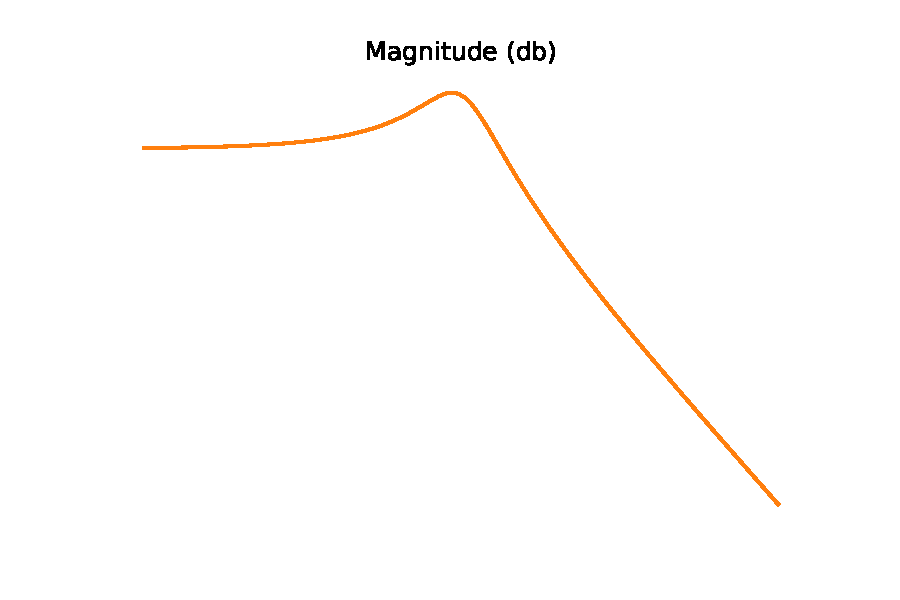
\includegraphics[width=\textwidth]{mag.pdf} 
            \caption{Magnitude} 
        \end{subfigure}~ 
        \begin{subfigure}[htbp]{0.5\textwidth} 
            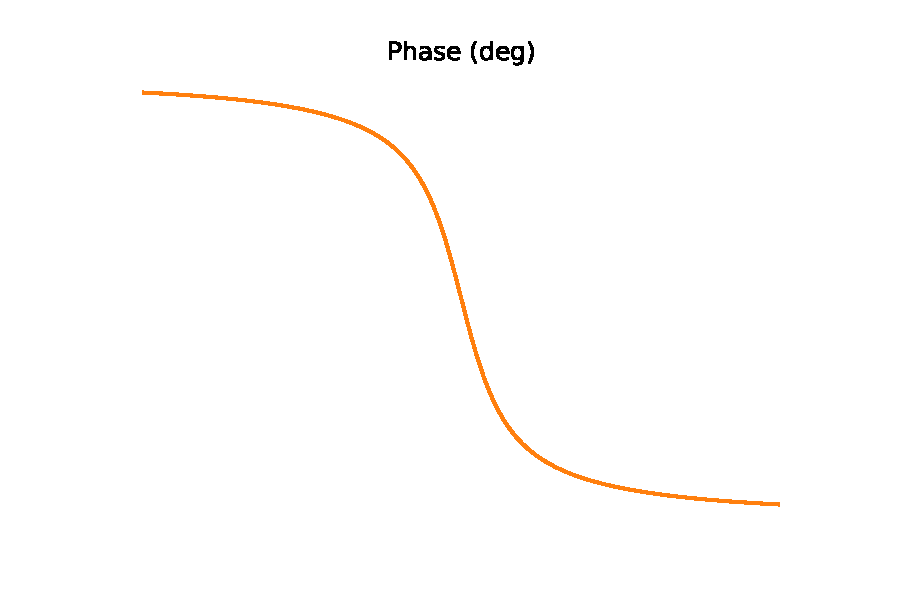
\includegraphics[width=\textwidth]{phase.pdf} 
            \caption{Phase} 
        \end{subfigure}
        \end{figure}
\end{enumerate}
\end{document}  